\documentclass[12pt,letterpaper,reqno]{article}

% \usepackage{mathtools}
\usepackage{epsfig}
\usepackage{amsmath}
\usepackage{amssymb}
\usepackage{amsthm}
\usepackage{indentfirst}
\usepackage{xspace}
\usepackage{multirow}
\usepackage{hyperref}
\usepackage{xcolor}
\usepackage{verbatim}
\usepackage[letterpaper,margin=1in,headheight=15pt]{geometry}
\usepackage{mathpazo}
\usepackage{tikz-cd}
\usepackage{booktabs}
\usepackage{framed}
\usepackage{float}
\usepackage{thmtools}
\usepackage{dashrule}
\usepackage[missing=]{gitinfo2}
\usepackage{fancyhdr}
\usepackage{enumerate}
\usepackage{graphicx}
\usepackage{mathrsfs}
\usepackage{calligra}
\usepackage[titletoc,title]{appendix}

\definecolor{darkblue}{rgb}{0.1,0.1,0.7}
\definecolor{darkred}{rgb}{0.5,0.1,0.1}
\definecolor{darkgreen}{rgb}{0.0,0.42,0.06}
\hypersetup{colorlinks=true,urlcolor=darkred,linkcolor=darkblue,citecolor=darkred}
\definecolor{shadecolor}{rgb}{0.85,0.85,0.85}

% Bibliography formatting
\usepackage[bibstyle=authoryear-comp,labeldate=false,defernumbers=true,maxnames=20,uniquename=init,dashed=false,backend=biber,sorting=none]{biblatex}

\DeclareNameAlias{sortname}{first-last}

\DeclareFieldFormat{url}{\url{#1}}
\DeclareFieldFormat[article]{pages}{#1}
\DeclareFieldFormat[inproceedings]{pages}{\lowercase{pp.}#1}
\DeclareFieldFormat[incollection]{pages}{\lowercase{pp.}#1}
\DeclareFieldFormat[article]{volume}{\textbf{#1}}
\DeclareFieldFormat[article]{number}{(#1)}
\DeclareFieldFormat[article]{title}{\MakeCapital{#1}}
\DeclareFieldFormat[inproceedings]{title}{#1}
\DeclareFieldFormat{shorthandwidth}{#1}

% Don't use "In:" in bibliography. Omit urls from journal articles.
\DeclareBibliographyDriver{article}{%
  \usebibmacro{bibindex}%
  \usebibmacro{begentry}%
  \usebibmacro{author/editor}%
  \setunit{\labelnamepunct}\newblock
  \MakeSentenceCase{\usebibmacro{title}}%
  \newunit
  \printlist{language}%
  \newunit\newblock
  \usebibmacro{byauthor}%
  \newunit\newblock
  \usebibmacro{byeditor+others}%
  \newunit\newblock
  \printfield{version}%
  \newunit\newblock
%  \usebibmacro{in:}%
  \usebibmacro{journal+issuetitle}%
  \newunit\newblock
  \printfield{note}%
  \setunit{\bibpagespunct}%
  \printfield{pages}
  \newunit\newblock
  \usebibmacro{eprint}
  \newunit\newblock
  \printfield{addendum}%
  \newunit\newblock
  \usebibmacro{pageref}%
  \usebibmacro{finentry}}

% Remove dot between volume and number in journal articles.
\renewbibmacro*{journal+issuetitle}{%
  \usebibmacro{journal}%
  \setunit*{\addspace}%
  \iffieldundef{series}
    {}
    {\newunit
     \printfield{series}%
     \setunit{\addspace}}%
  \printfield{volume}%
%  \setunit*{\adddot}%
  \printfield{number}%
  \setunit{\addcomma\space}%
  \printfield{eid}%
  \setunit{\addspace}%
  \usebibmacro{issue+date}%
  \newunit\newblock
  \usebibmacro{issue}%
  \newunit}


% Bibliography categories
\def\makebibcategory#1#2{\DeclareBibliographyCategory{#1}\defbibheading{#1}{\section*{#2}}}
\makebibcategory{books}{Books}
\makebibcategory{papers}{Refereed research papers}
\makebibcategory{chapters}{Book chapters}
\makebibcategory{conferences}{Papers in conference proceedings}
\makebibcategory{techreports}{Unpublished working papers}
\makebibcategory{bookreviews}{Book reviews}
\makebibcategory{editorials}{Editorials}
\makebibcategory{phd}{PhD thesis}
\makebibcategory{subpapers}{Submitted papers}
\makebibcategory{curpapers}{Current projects}

\setlength{\bibitemsep}{2.65pt}
\setlength{\bibhang}{.8cm}
\renewcommand{\bibfont}{\small}

\renewcommand*{\bibitem}{\addtocounter{papers}{1}\item \mbox{}\hskip-0.85cm\hbox to 0.85cm{\hfill\arabic{papers}.~~}}
\defbibenvironment{bibliography}
{\list{}
  {\setlength{\leftmargin}{\bibhang}%
   \setlength{\itemsep}{\bibitemsep}%
   \setlength{\parsep}{\bibparsep}}}
{\endlist}
{\bibitem}

\newenvironment{publications}{\section{\LARGE Publications}\label{papersstart}\vspace*{0.2cm}\small
\titlespacing{\section}{0pt}{1.5ex}{1ex}\itemsep=0.00cm
}{\label{papersend}\addtocounter{sumpapers}{-1}\refstepcounter{sumpapers}\label{sumpapers}}

\def\printbib#1{\printbibliography[category=#1,heading=#1]\lastref{sumpapers}}

% Counters for keeping track of papers
\newcounter{papers}\setcounter{papers}{0}
\newcounter{sumpapers}\setcounter{sumpapers}{0}
\def\lastref#1{\addtocounter{#1}{\value{papers}}\setcounter{papers}{0}}

% theorem environments
\declaretheoremstyle[spaceabove=0.25cm,spacebelow=0.25cm,notefont=\normalfont\bfseries, notebraces={(}{)}]{theorem}
\declaretheoremstyle[spaceabove=0.25cm,spacebelow=0.25cm,bodyfont=\normalfont,notefont=\normalfont\bfseries, notebraces={(}{)}]{noital}
\declaretheoremstyle[spaceabove=0.25cm,spacebelow=0.25cm,bodyfont=\normalfont\color{darkgreen},notefont=\normalfont\bfseries, notebraces={(}{)}]{green}
\declaretheoremstyle[spaceabove=0.25cm,spacebelow=0.25cm,bodyfont=\normalfont,notefont=\normalfont\bfseries,qed=$\qedsymbol$,notebraces={(}{)}]{proofstyle}

\declaretheorem[name=Theorem,numberwithin=section,style=theorem]{thm}
\declaretheorem[name=Proposition,sibling=thm,style=theorem]{prop}
\declaretheorem[name=Corollary,sibling=thm,style=theorem]{cor}
\declaretheorem[name=Lemma,sibling=thm,style=theorem]{lem}
\declaretheorem[name=Definition,sibling=thm,style=noital]{defn}
\declaretheorem[name=Example,sibling=thm,style=noital]{example}
\declaretheorem[name=Exercise,numberwithin=section,style=green]{exercise}
\declaretheorem[name=Proof,style=proofstyle,numbered=no]{pf}
\declaretheorem[name=Solution,style=proofstyle,numbered=no]{solution}
\numberwithin{equation}{section}


% macros for convenience
\newcommand{\tops}{\texorpdfstring}

\newcommand{\nid}{\noindent}

\newcommand{\fa}{{\mathfrak a}}
\newcommand{\fp}{{\mathfrak p}}
\newcommand{\fk}{{\mathfrak k}}
\newcommand{\fg}{{\mathfrak g}}
\newcommand{\fh}{{\mathfrak h}}
\newcommand{\fn}{{\mathfrak n}}
\newcommand{\fq}{{\mathfrak q}}
\newcommand{\fm}{{\mathfrak m}}
\newcommand{\fr}{{\mathfrak r}}
\newcommand{\fu}{{\mathfrak u}}
\newcommand{\fG}{{\mathfrak G}}

\newcommand{\cC}{\ensuremath{\mathcal C}}
\newcommand{\cG}{\ensuremath{\mathcal G}}
\newcommand{\cB}{\ensuremath{\mathcal B}}
\newcommand{\cL}{\ensuremath{\mathcal L}}
\newcommand{\cS}{\ensuremath{\mathcal S}}
\newcommand{\cF}{\ensuremath{\mathcal F}}
\newcommand{\cK}{\ensuremath{\mathcal K}}
\newcommand{\cZ}{\ensuremath{\mathcal Z}}
\newcommand{\cM}{\ensuremath{\mathcal M}}
\newcommand{\cN}{\ensuremath{\mathcal N}}
\newcommand{\cO}{\ensuremath{\mathcal O}}
\newcommand{\cH}{\ensuremath{\mathcal H}}
\newcommand{\cX}{\ensuremath{\mathcal X}}
\newcommand{\cY}{\ensuremath{\mathcal Y}}
\newcommand{\cA}{\ensuremath{\mathcal A}}
\newcommand{\cI}{\ensuremath{\mathcal I}}

\newcommand{\R}{\ensuremath{\mathbb R}}
\newcommand{\C}{\ensuremath{\mathbb C}}
\newcommand{\PP}{\ensuremath{\mathbb P}}
\newcommand{\Z}{\ensuremath{\mathbb Z}}
\newcommand{\Q}{\ensuremath{\mathbb Q}}
\newcommand{\A}{\ensuremath{\mathbb A}}
\newcommand{\bbH}{\ensuremath{\mathbb H}}
\newcommand{\bbI}{\ensuremath{\mathbb I}}
\newcommand{\bS}{\ensuremath{\mathbb S}}

\newcommand{\half}{\ensuremath{\frac{1}{2}}}
\newcommand{\qtr}{\ensuremath{\frac{1}{4}}}
\newcommand{\bq}{{\mathbf q}}
\newcommand{\N}{{\mathcal N}}
\newcommand{\F}{{\mathcal F}}
\newcommand{\HH}{{\mathcal H}}
\newcommand{\LL}{{\mathcal L}}
\newcommand{\RR}{{\mathcal R}}
\newcommand{\V}{{\mathcal V}}
\newcommand{\dirac}{\!\!\not\!\partial}
\newcommand{\Dirac}{\!\!\not\!\!D}
\newcommand{\cE}{{\mathcal E}}
\newcommand{\vs}{\not\!v}
\newcommand{\kahler}{K\"ahler\xspace}
\newcommand{\kq}{/\!\!/}
\newcommand{\kql}[1]{/\!\!/\!\!_#1\,}
\newcommand{\hk}{hyperk\"ahler\xspace}
\newcommand{\Hk}{Hyperk\"ahler\xspace}
\newcommand{\hkq}{/\!\!/\!\!/\!\!/}
\newcommand{\hkql}[1]{/\!\!/\!\!/\!\!/\!\!_#1\,}
\newcommand{\del}{\ensuremath{\partial}}
\newcommand{\delbar}{\ensuremath{\overline{\partial}}}
\newcommand{\bl}{{\bf L}}
\newcommand{\J}{{\mathrm j}}
\newcommand{\K}{{\mathrm k}}
\newcommand{\e}{{\mathrm e}}
\newcommand\bid{{\mathbf 1}}
\newcommand{\de}{\mathrm{d}}
\newcommand{\ab}{\mathrm{ab}}
\newcommand{\vol}{\mathrm{vol}}
\renewcommand{\sf}{\mathrm{sf}}
\newcommand{\inst}{\mathrm{inst}}
\newcommand{\eff}{\mathrm{eff}}
\newcommand{\dR}{\mathrm{dR}}
\newcommand{\closed}{\mathrm{closed}}
\newcommand{\exact}{\mathrm{exact}}

\newcommand{\abs}[1]{\lvert#1\rvert}
\newcommand{\norm}[1]{\lVert#1\rVert}
\newcommand{\IP}[1]{\langle#1\rangle}
\newcommand{\DIP}[1]{\langle\!\langle#1\rangle\!\rangle}
\newcommand{\dwrt}[1]{\frac{\partial}{\partial#1}}
\newcommand{\eps}{\epsilon}
\newcommand{\simarrow}{\xrightarrow\sim}

\newcommand{\mmaref}[1]{}

\newcommand{\ti}[1]{\textit{#1}}
\newcommand{\tb}[1]{\textbf{#1}}
\newcommand{\lo}{\text{\calligra o}\,}
\newcommand{\dd}{\ensuremath{\mathscr{D}}}
\newcommand{\bu}{{\bf u}}
\newcommand{\bv}{{\bf v}}
\newcommand{\bw}{{\bf w}}
\newcommand{\bx}{{\bf x}}
\newcommand{\by}{{\bf y}}
\newcommand{\bz}{{\bf z}}
\newcommand{\ba}{{\bf a}}
\newcommand{\bb}{{\bf b}}
\newcommand{\bbr}{{\bf r}}
\newcommand{\bff}{{\bf f}}
\newcommand{\bgg}{{\bf g}}
\newcommand{\bt}{{\bf t}}
\newcommand{\bn}{{\bf n}}
\newcommand{\ii}{{\bf {\hat{i}}}}
\newcommand{\jj}{{\bf {\hat{j}}}}
\newcommand{\kk}{{\bf {\hat{k}}}}


\DeclareMathOperator{\ad}{ad}
\DeclareMathOperator{\im}{Im}
\DeclareMathOperator{\re}{Re}
\DeclareMathOperator{\Tr}{Tr}
\DeclareMathOperator{\End}{End}
\DeclareMathOperator{\Hom}{Hom}
\DeclareMathOperator{\Aut}{Aut}
\DeclareMathOperator{\Sym}{Sym}
\DeclareMathOperator{\Lie}{Lie}
\DeclareMathOperator{\diag}{diag}
\DeclareMathOperator{\Bun}{Bun}
\DeclareMathOperator{\Vect}{Vect}
\DeclareMathOperator{\Span}{Span}
\DeclareMathOperator{\grad}{grad}
\DeclareMathOperator{\rank}{rank}
\DeclareMathOperator{\ind}{ind}
\DeclareMathOperator{\coker}{coker}
\DeclareMathOperator{\Jac}{Jac}
\DeclareMathOperator{\Hol}{Hol}
\DeclareMathOperator{\gr}{gr}

\newcommand{\insfig}[2]{

\medskip
\noindent
\begin{minipage}{\linewidth}

\makebox[\linewidth]{\includegraphics[keepaspectratio=true,scale=#2]{figures/#1-crop.pdf}}

\end{minipage}
\medskip

}


% \newcommand{\insfig}[2]{\begin{figure}[htbp] \centering \includegraphics[scale=#2]{figures/#1-crop.pdf} \label{fig:#1} \end{figure}}
% syntax: \insfig{name}{0.5}{caption}

\newcommand{\fixme}[1]{{\color{orange}{[#1]}}}
\newcommand{\currentposition}{{\color{blue} \noindent\makebox[\linewidth]{\hdashrule{\paperwidth}{1pt}{3mm}}}}

% \mathtoolsset{showonlyrefs}

\bibliography{mvc}

\begin{document}
\pagestyle{fancy}
\lhead{{\tiny \color{gray} \tt \gitAuthorIsoDate}}
\chead{\tiny \ti{Multivariable Calculus, GSMST Spring 2020}}
\rhead{{\tiny \color{gray} \tt \gitAbbrevHash}}
\renewcommand{\headrulewidth}{0.5pt}


\begin{center}
\tb{Multivariable Calculus} \\
Anderson Trimm \\
Gwinnett School of Mathematics, Science and Technology \\
\end{center}

{These are the notes for the Spring Semester 2020
course in Multivariable Calculus at GSMST. They will continually be updated throughout the course. The latest PDF can always be accessed
at \small \url{https://github.com/atrimm/mvc/blob/master/Course%20Notes/multivariable_calculus_2020.pdf.}

\tableofcontents
\renewcommand{\listtheoremname}{Quick reference}
\listoftheorems[onlynamed]

\newpage

%\setcounter{page}{1}

\section{Curves in Spaces}
In this section we study functions with one input and multiple outputs.

\subsection{Vector-valued functions}
\subsubsection{Definitions}
Suppose a particle moves in the plane along the following curve $C$:
	\begin{center}
		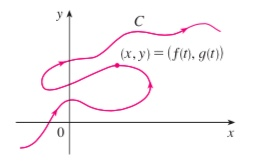
\includegraphics[scale=0.5]{figures_mvc/plane_curve}
	\end{center}
Since the curve fails the vertical line test, $C$ cannot be described as the graph of a function $y=f(x)$. Note however that the x- and y-coords of the particle are functions of time
\begin{align*}
	x=f(t), \hspace{0.5cm} y=g(t)
\end{align*}
so the curve $C$ can be described as the image of function ${\bf r}:I \to \mathbb{R}^2$ defined by 
\begin{align*}
	\bbr(t)=(f(t),g(t)),
\end{align*}
where $I=[a,b]$ is an interval in $\R$. \fixme{Add mapping diagram.}

\begin{defn}[Vector-valued function]
Let $U \subseteq \R$. A mapping $\bbr:U \to \mathbb{R}^n$ called a \emph{vector-valued function}. The value of $\bbr$ at $t \in U$ can be written as
\begin{align*}
	\bbr(t)=(r_1(t),r_2(t),\dots,r_n(t))
\end{align*}
where the $n$ functions $r_i:U \to \R$, $i=1,\dots,n$ are called the \emph{component functions} of $\bbr$.	
\end{defn}
Unless specified otherwise, we will take the domain $U$ of a vector-valued function to be the largest domain on which all of the component functions are defined.
\begin{example}
Consider the vector-valued function $\bbr:U \to \mathbb{R}^3$ defined by
	\begin{align*}
		\bbr(t)=(t^3,\ln(3-t),\sqrt{t}).
	\end{align*}
The component functions of $\bbr(t)$ are 
\begin{align*}
	r_1(t)=t^3, \hspace{0.5cm} r_2(t)=\ln(3-t), \hspace{0.5cm} r_3(t)=\sqrt{t}.
\end{align*}
The domains of each of these functions, respectively, are 
\begin{align*}
	U_1=\R, \hspace{0.5cm} U_2=(-\infty,3), \hspace{0.5cm} U_3=[0,\infty),
\end{align*}	
so the domain $U$ of $\bbr(t)$ is 
\begin{align*}
	U=U_1 \cap U_2 \cap U_3=[0,3).
\end{align*} 
\end{example}

\begin{exercise}
	Consider the vector-valued function $\bbr:U \to \mathbb{R}^3$ defined by
	\begin{align*}
		\bbr(t)=\left(\frac{t-2}{t+2},\sin t, \ln(9-t^2)\right).
	\end{align*}
What is the domain $U$ of the function?
\end{exercise}
{\color{red}\begin{solution}
	The component functions of $\bbr(t)$ are 
	\begin{align*}
		r_1=\frac{t-2}{t+2}, \hspace{0.5cm} r_2=\sin t, \hspace{0.5cm} r_3=\ln(9-t^2).
	\end{align*}
	The domains of $r_1(t)$ and $r_2(t)$ are given, respectively, by
	\begin{align*}
		U_1=(-\infty,2) \cup (2,\infty), \hspace{0.5cm} U_2=\R.
	\end{align*}
	To find the domain of $r_3(t)$, we need to solve the inequality
	\begin{align*}
		9-t^2>0. \\
	\end{align*}
	The graph of the function $y=9-x^2$ is a concave-down parabola with $y$-intercept 9 and $x$-intercepts $\pm 3$. 
	
	\begin{figure}[h]
	\begin{center}
		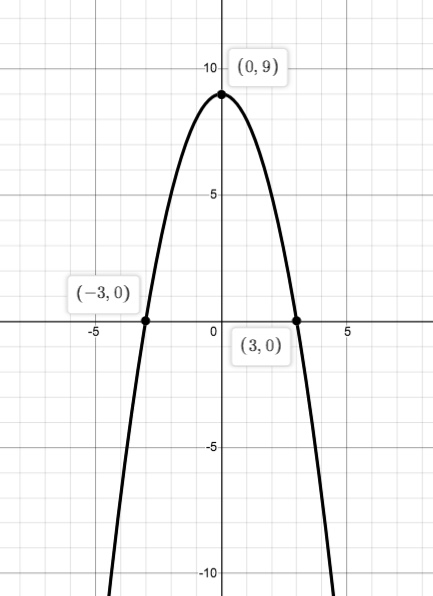
\includegraphics[scale=0.3]{figures_mvc/parab_down}
	\end{center}
	\caption{Graph of $y=9-x^2$.}
\end{figure}
	We have $y>0$ where the graph is above the $x$-axis, so $y>0$ when $-3<x<3$. The domain of $r_3(t)$ is therefore
	\begin{align*}
		U_3=(-3,3).
	\end{align*}
	The domain of $\bbr(t)$ is then
	\begin{align*}
		U=U_1 \cap U_2 \cap U_3=(-3,-2)\cup (-2,3).
	\end{align*}
\end{solution}}

\subsubsection{Review: limits of single-variable functions}
Before considering limits of vector-valued functions, let's review the definition for a real-valued function $y=f(x)$ of a single real variable $x$.

To motivate the definition, consider the function
\begin{align*}
	f(x)=\begin{cases}
		2x-1, \ \text{ if } x \neq 3 \\
		6, \hspace{1.0cm} \text{ if } x = 3 \\
	\end{cases}
\end{align*}
whose graph is shown in the figure below.

\begin{figure}[h]\label{fig:lim_def}
	\begin{center}
		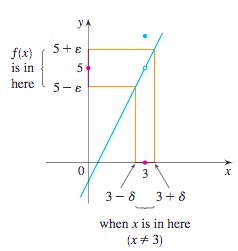
\includegraphics[scale=0.7]{figures_mvc/graph_limit_defn}
	\end{center}
	\caption{Graph of the function $y=f(x)$ in the example above.}
\end{figure}
From the graph, we see that when $x$ is close to 3 but not equal to 3, then $f(x)$ is close to 5, and so $\lim_{x \to 3}f(x)=5$.

To obtain more detailed information about how $f(x)$ varies when $x$ is close to 3, we ask the following question: 

\emph{How close to 3 does $x$ have to be so that $f(x)$ differs from 5 by less than $0.1$?}

The distance from $x$ to $3$ is $|x-3|$ and the distance from $f(x)$ to 5 is $|f(x)-5|$, so our problem is to find a number $\delta$ such that 
\begin{align*}
	|f(x)-5|<0.1 \hspace{0.5cm} \text{ if } \hspace{0.5cm} 0<|x-3|<\delta.
\end{align*}
If $x \neq 3$, then 
\begin{align*}
	|f(x)-5|=|(2x-1)-5|=|2x-6|=2|x-3|
\end{align*}
so we see that by taking $\delta=\frac{1}{2}(0.1)=0.05$, we have $|f(x)-5|<2(0.05)=0.1$. Thus, an answer to the problem is given by $\delta=0.05$; that is, if $x$ is within a distance of $0.05$ from 3, then $f(x)$ will be within a distance of $0.1$ from 5.

If we change the number $0.1$ in our problem to the smaller number $0.01$, then by using the same method we find that $f(x)$ will differ from 5 by less than $0.01$ provided that $x$ differs from 3 by less than $\frac{1}{2}(0.01)=0.005$; that is,
\begin{align*}
	|f(x)-5|<0.01 \hspace{0.5cm} \text{ if } \hspace{0.5cm} 0<|x-3|<0.005.
\end{align*}
Similarly,
\begin{align*}
	|f(x)-5|<0.001 \hspace{0.5cm} \text{ if } \hspace{0.5cm} 0<|x-3|<0.0005.
\end{align*}
Think of the numbers $0.1, 0.01, 0.001$ above as \emph{error tolerances} that we might allow. That is, when challenged with an error tolerance, it is our task to find a corresponding $\delta$ so that whenever $x$ is within a distance of $\delta$ from 3, $f(x)\approx 5$, within the given error tolerance. 

Now for 5 to be the precise limit of $f(x)$ as $x$ approaches 3, we must not only be able to bring the difference between $f(x)$ and 5 below each of these numbers; we must be able to bring it below \emph{any} positive number. And, by exactly the same reasoning, we can. That is, if $\epsilon$ is any positive number, then by choosing $\delta=\frac{\epsilon
}{2}$, we find
\begin{align}\label{eq:review_limit_example}
	|f(x)-5|<\epsilon \hspace{0.5cm} \text{ if } \hspace{0.5cm} 0<|x-3|<\delta=\frac{\epsilon}{2}.
\end{align}
This is a precise way of saying that $f(x)$ is close to 5 when $x$ is close to 3, because Equation \eqref{eq:review_limit_example} says that we can make the values of $f(x)$ within an arbitrary distance $\epsilon$ from 5 by taking the values of $x$ within a distance $\frac{\epsilon}{2}$ from 3 (but $x \neq 3$).

Note that Equation \eqref{eq:review_limit_example} can be rewritten as follows:
\begin{align*}
	\text{ if } \hspace{0.5cm} 3-\delta<x<3+\delta \hspace{0.2cm} (x \neq 3) \hspace{0.5cm} \text{ then } \hspace{0.5cm} 5-\epsilon<f(x)<5+\epsilon
\end{align*}
as illustrated in the figure above. This says that by taking the values of $x$ ($x \neq 3$) to lie in the interval $(3-\delta,3+\delta)$ we can make the values of $f(x)$ lie in the interval $(5-\epsilon,5+\epsilon)$.

Following the reasoning in this example,  the precise definition of a limit is the following.

\begin{defn}[Limit of a single-variable function]\label{def:limit_of_a_single-variable_function}
	Let $(a,b)$ be an open interval containing the point $x_0$ and let $f(x)$ be a real-valued function defined on this interval, except possibly at $x_0$ itself. A number $L$ is called the \emph{limit of $f(x)$ as $x$ approaches $x_0$} if for every $\epsilon>0$ there exists a $\delta>0$ such that $|f(x)-L|<\epsilon$ whenever $0<|x-x_0|<\delta$. If such an $L$ exists, we write
	\begin{align*}
		\lim_{x \to x_0}f(x)=L.
	\end{align*}
\end{defn}

\begin{thm}[Uniqueness of limits]\label{thm:uniqueness_of_limits}
	If $f(x)$ has a limit $L$ at $x_0$, then the limit is unique.
\end{thm}

\begin{pf}
Suppose that $\lim_{x \to x_0}f(x)=L$ and $\lim_{x \to x_0}f(x)=L'$. Then, given any $\epsilon>0$ there exist positive numbers $\delta_1$ and $\delta_2$ such that 
\begin{align*}
	|f(x)-L|<\frac{\epsilon}{2} \hspace{0.5cm} \text{ if } \hspace{0.5cm} |x-x_0|<\delta_1
\end{align*} 	
and
\begin{align*}
	|f(x)-L'|<\frac{\epsilon}{2} \hspace{0.5cm} \text{ if } \hspace{0.5cm} |x-x_0|<\delta_2.
\end{align*} 
Then by taking $|x-x_0|<\delta=\min\{\delta_1,\delta_2\}$, we have
\begin{align*}
	|L-L'|=|L-L'+f(x)-f(x)|=|L-f(x)+f(x)-L|\leq |f(x)-L|+|f(x)-L'|<\frac{\epsilon}{2}+\frac{\epsilon}{2}=\epsilon.
\end{align*}
For this to be true for all $\epsilon>0$, we must have $L-L'=0$, or $L=L'$.
\end{pf}


\begin{exercise}
Use Definition \ref{def:limit_of_a_single-variable_function} to prove that $\lim_{x \to 3}(4x-5)=7$.
\end{exercise}

{\color{red} \begin{solution}
Let $\epsilon>0$. For all $x \neq 3$, 
\begin{align*}
	|f(x)-7|=|(4x-5)-7|=|4x-12|=4|x-3|.
\end{align*} 
By taking $\delta=\frac{\epsilon}{4}$, we have $0<|x-3|<\frac{\epsilon}{4}$ and therefore
\begin{align*}
	|f(x)-7|=4|x-3|<4\cdot \frac{\epsilon}{4}=\epsilon,
\end{align*}	
which proves that $\lim_{x \to 3}(4x-5)=7$.
\end{solution}}

\begin{example}
We now use Definition \ref{def:limit_of_a_single-variable_function} to prove that $\lim_{x \to 3}x^2=9$.	

Let $\epsilon>0$. For all $x \neq 3$, we have
\begin{align*}
	|f(x)-9|=|x^2-9|=|(x+3)(x-3)|=|x+3||x-3|.
\end{align*} 
Notice that if we can find a positive number $C$ such that $|x+3|<C$, then
\begin{align*}
	|x+3||x-3|<C|x-3|
\end{align*}
and we can make $C|x-3|<\epsilon$ by taking $|x-3|<\frac{\epsilon}{C}=\delta$. We can find such a number $C$ if we restrict $x$ to lie in some interval centered at 3. Since we are only interested in values of $x$ that are close to 3, this is exactly what we want. Let's assume that $|x-3|<\alpha$ for some positive number $\alpha$, say $\alpha=1$ (it does not matter what number we take here). Then we have
\begin{align*}
	x-3<1 \hspace{0.5cm} \text{ or }  \hspace{0.5cm} -x+3<1.
\end{align*}
The first inequality says $x<4$ and the second says $2<x$, so $|x-3|<1$ implies that 
\begin{align*}
	2<x<4.
\end{align*}
Adding 3 to both sides of this inequality gives 
\begin{align*}
	5<x+3<7,
\end{align*}
and therefore $|x+3|<|7|=7=C$. But now there are two restrictions on $|x-3|$, namely
\begin{align*}
	|x-3|<1 \hspace{0.5cm} \text{ and } \hspace{0.5cm} |x-3|<\frac{\epsilon}{C}=\frac{\epsilon}{7}.
\end{align*}
To make sure that both of these inequalities are satisfied, we take $\delta=\min\{1,\frac{\epsilon}{7}\}$. Since $0<|x-3|<\delta$ implies $|x^2-9|<\epsilon$, this proves that $\lim_{x \to 3}x^2=9$.
\end{example}
The previous example shows that it is not always easy to prove that a function has a particular limit using Definition \ref{def:limit_of_a_single-variable_function}. In fact, if we had considered a more complicated function such as 
\begin{align*}
	f(x)=\frac{6x^2-8x+9}{2x^2-1}
\end{align*}
then proving that $\lim_{x \to 1}f(x)=7$ using Definition \ref{def:limit_of_a_single-variable_function} would require a great deal of ingenuity. Instead, we prove the following theorems, which makes evaluating limits much easier.

\begin{lem}[Triangle Inequality]\label{lem:triangle_inequality}
	For all $x,y \in \R$, 
	\begin{align*}
		|x+y| \leq |x|+|y|.
	\end{align*}
\end{lem}

\begin{pf}
We have
\begin{align*}
	|x+y|^2=(x+y)^2&=x^2+y^2+2xy \\
	&=|x|^2+|y|^2+2xy \\
	&\leq |x|^2+|y|^2+2|x||y| \\
	&=(|x|+|y|)^2.
\end{align*}	
Since both sides are nonnegative, this implies that 
\begin{align*}
	|x+y| \leq |x|+|y|.
\end{align*}
\end{pf}



\begin{thm}[Limit laws for single-variable functions]\label{thm:limit_laws_for_single-variable_functions}
Suppose $f(x)$ and $g(x)$ are defined on the same open set containing $x_0$, and that 
\begin{align*}
	\lim_{x \to x_0}f(x)=L \hspace{0.5cm} \text{ and } \hspace{0.5cm} \lim_{x \to x_0}g(x)=M.
\end{align*}
Then
	\begin{enumerate}[(i)]
		\item $\lim_{x \to x_0}c=c$ for any constant $c \in \R$.
		\item $\lim_{x \to x_0}x=x_0$.
		\item $\lim_{x \to x_0} cf(x)=cL$ for any $c \in \R$;
		\item $\lim_{x \to x_0}(f(x)+ g(x))=L+M$;
		\item $\lim_{x \to x_0}(f(x)g(x))=LM$;
		\item $\lim_{x \to x_0}=\frac{f(x)}{g(x)}=\frac{L}{M}$ whenever $M \neq 0$.
	\end{enumerate}
\end{thm}

\begin{pf}
\begin{enumerate}[(i)]
	\item Let $\epsilon>0$. Since $|c-c|=0$, $|c-c|<\epsilon$ whenever $|x-x_0|<\delta$ for any positive number $\delta$.
	\item Given $\epsilon>0$, by taking $\delta=\epsilon$ we have $|x-x_0|<\epsilon$ whenever $|x-x_0|<\delta=\epsilon$.
	\item Since $\lim_{x \to x_0}f(x)=L$, given $\epsilon>0$ there exists a corresponding $\delta>0$ such that $|f(x)-L|<\epsilon$ whenever $0<|x-x_0|<\delta$. Then $|cf(x)-cL|=|c||f(x)-L|<\epsilon$ whenever $0<|x-x_0|<\frac{\epsilon}{|c|}$.
	\item We have
	\begin{align*}
		|f(x)+g(x)-(L+M)|=|(f(x)-L)+(g(x)-M)| \leq |f(x)-L|+|g(x)-M|
	\end{align*}
	by the Triangle Inequality (Lemma \ref{lem:triangle_inequality}). Since $\lim_{x \to x_0}f(x)=L$ and $\lim_{x \to x_0}g(x)=M$, given $\epsilon>0$ there exist positive numbers $\delta_1$ and $\delta_2$ such that 
	\begin{align*}
		|f(x)-L|<\frac{\epsilon}{2} \hspace{0.5cm} \text{ if } \hspace{0.5cm} |x-x_0|<\delta_1
	\end{align*} 
	and 
	\begin{align*}
		|g(x)-M|<\frac{\epsilon}{2} \hspace{0.5cm} \text{ if } \hspace{0.5cm} |x-x_0|<\delta_2.
	\end{align*} 
	By taking $|x-x_0|<\delta=\min\{\delta_1,\delta_2\}$, we have 
	\begin{align*}
		|f(x)+g(x)-(L+M)|\leq |f(x)-L|+|g(x)-M|<\frac{\epsilon}{2}+\frac{\epsilon}{2}=\epsilon,
	\end{align*}
	which proves that $\lim_{x \to x_0}(f(x)+g(x))=L+M$.
	\item First, note that
		\begin{align*}
			f(x)g(x)-LM&=(f(x)-L)(g(x)-M)+L(g(x)-M)+M(f(x)-L).
		\end{align*} 
		Let $\epsilon>0$. Since $\lim_{x \to x_0}f(x)=L$ there exists $\delta_1>0$ such that $|f(x)-L|<\sqrt{\epsilon}$ whenever $|x-x_0|<\delta_1$. Since $\lim_{x \to x_0}g(x)=M$ there exists $\delta_2>0$ such that $|g(x)-M|<\sqrt{\epsilon}$ whenever $|x-x_0|<\delta_2$. Then, whenever $|x-x_0|<\delta=\min\{\delta_1,\delta_2\}$, we have
		\begin{align*}
			|(f(x)-L)(g(x)-M)|=|f(x)-L||g(x)-M|<(\sqrt{\epsilon})^2=\epsilon
		\end{align*}
		which shows that $\lim_{x-x_0}(f(x)-L)(g(x)-M)=0$. By (iii), 
		\begin{align*}
			\lim_{x \to x_0}L(g(x)-M)=L\lim_{x \to x_0}(g(x)-M)=L\cdot0=0,
		\end{align*}
		 and 
		\begin{align*}
			\lim_{x \to x_0}M(f(x)-L)=M\lim_{x \to x_0}(f(x)-L)=M\cdot0=0.
		\end{align*}
		Applying (iv),
		\begin{align*}
			\lim_{x \to x_0}(f(x)g(x)-LM)&=\lim_{x \to x_0}(f(x)-L)(g(x)-M)+\lim_{x \to x_0}L(g(x)-M)+\lim_{x \to x_0}M(f(x)-L) \\
			&=0+0+0 \\
			&=0,
		\end{align*}
		and therefore
		\begin{align*}
			\lim_{x \to x_0}f(x)g(x)=LM.
		\end{align*}
	\item First, note that since $|M|>0$ and $\lim_{x \to x_0}g(x)=M$, there exists $\delta_1>0$ such that $|g(x)|>\frac{1}{2}|M|$ whenever $|x-x_0|<\delta_1$ \fixme{Draw a picture.}. Let $\epsilon>0$. Choose $\delta_2>0$ such that $|x-x_0|<\delta_2$ implies that $|g(x)-M|<\frac{1}{2}|M|^2\epsilon$. Then, for $|x-x_0|<\delta = \min\{\delta_1,\delta_2\}$, we have
	\begin{align*}
		|\frac{1}{g(x)}-\frac{1}{M}|&=|\frac{M-g(x)}{Mg(x)}|\\
		&=\frac{|g(x)-M|}{|Mg(x)|} \\
		&<\frac{\frac{1}{2}|M|^2\epsilon}{\frac{1}{2}|M|^2} \\
		&=\epsilon,	
	\end{align*}
	and therefore $\lim_{x \to x_0}\frac{1}{g(x)}=\frac{1}{M}$. It then follows from (v) that
	\begin{align*}
		\lim_{x \to x_0}\frac{f(x)}{g(x)}&=\lim_{x \to x_0}f(x) \lim_{x \to x_0}\frac{1}{g(x)} \\
		&=\frac{L}{M}.
	\end{align*}
\end{enumerate}	
\end{pf}
Using Theorem \ref{thm:limit_laws_for_single-variable_functions}, it is much easier to prove the limits in the examples above. For instance
\begin{align*}
	\lim_{x \to 3}(4x-5)&=(\lim_{x \to 3}4)(\lim_{x \to 3}x)+(\lim_{x \to 3}(-5)) \\
	&=4(3)+(-5) \\
	&=12-5 \\
	&=7,
\end{align*}
and 
\begin{align*}
	\lim_{x \to 3}x^2=(\lim_{x \to 3}x)(\lim_{x \to 3}x)=(3)(3)=9.
\end{align*}
Note that, in both of these examples, the function $f(x)$ is actually defined at $x_0$ and $\lim_{x \to x_0}f(x)=f(x_0)$; that is, the limit of $f(x)$ as $x$ approaches $x_0$ is equal to the value of $f(x)$ at $x_0$.

\begin{defn}[Continuity]
	Let $f(x)$ be defined on an open interval $(a,b)$ containing a point $x_0$. We say that $f(x)$ is \emph{continuous at $x_0$} if $\lim_{x \to x_0}f(x)=f(x_0)$. We then say that $f(x)$ is \emph{continuous on $(a,b)$} if $f(x)$ is continuous at every point in $(a,b)$.
\end{defn}
The limit laws in Theorem \ref{thm:limit_laws_for_single-variable_functions} imply that
\begin{itemize}
	\item Polynomials are continuous on $\R$;
	\item Rational functions are continuous wherever they are defined;
	\item The absolute value function $f(x)=|x|$ is continuous;
\end{itemize}
Trig functions, and exponential and logarithmic functions are all also continuous wherever they are defined.

\begin{exercise}
Prove that $f(x)=|x|$ is continuous on $\R$.	
\end{exercise}

{\color{red} \begin{solution}
 	If $x>0$, then $f(x)=x$ which is continuous since it is a polynomial. The same is true for $x<0$ since then $f(x)=-x$. By taking $\delta=\epsilon$, $|f(x)-0|=||x||=|x|<\epsilon$ whenever $|x|<\delta=\epsilon$, so $\lim_{x \to 0}f(x)=0=f(0)$, which shows that $f(x)$ is also continuous at $x=0$. Thus, $f(x)$ is continuous on $\R$.
 \end{solution}}

\begin{thm}[New continuous functions from old]
	Let $f(x)$ and $g(x)$ be defined on the same open interval containing $x_0$. If $f(x)$ and $g(x)$ are continuous at $x_0$, then so are
	\begin{enumerate}[(i)]
		\item $cf(x)$
		\item \fixme{Finish.}
	\end{enumerate}
\end{thm}


\begin{thm}[A composition of continuous functions is continuous]\label{thm:a_composition_of_continuous_functions_is_continuous}
	Suppose $f(x)$ is defined on an open interval containing $x_0$ and  $g(x)$ is defined on an open interval containing $f(x_0)$. If $f$ is continuous at $x_0$ and $g(x)$ is continuous at $f(x_0)$, then $(g \circ f)(x)$ is continuous at $x_0$.
\end{thm}

\begin{pf}
Let $\epsilon>0$. Since $g$ is continuous at $f(x_0)$, corresponding to $\epsilon$ there exists $\eta>0$ such that $|g(f(x))-g(f(x_0))|<\epsilon$ whenever $|f(x)-f(x_0)|<\eta$. Since $f$ is continuous at $x_0$, corresponding to $\eta$ there exists $\delta>0$ such that $|f(x)-f(x_0)|<\eta$ whenever $|x-x_0|<\delta$. This shows that $|g(f(x))-g(f(x_0))|<\epsilon$ whenever $|x-x_0|<\delta$, proving that $(g \circ f)(x)$ is continuous at $x_0$.
\end{pf}

\begin{example}
Consider the function $f(x)=e^{x^2}$. We can view $f(x)$ as the composition $(h \circ g)(x)$, where $h(x)=e^x$ and $g(x)=x^2$. Since $h(x)$ and $g(x)$ are continuous on $\R$, by Theorem \ref{thm:a_composition_of_continuous_functions_is_continuous} so is $f(x)$.
\end{example}

\subsubsection{Limits of vector-valued functions}
Throughout this section, let $I=(a,b)$ denote an open interval in $\R$ containing a point $t_0$, and let $\bbr(t)$ be a vector-valued function defined on $I$, except perhaps at $t_0$ itself. 
\begin{defn}[Limit of a vector-valued function]
	A fixed vector $\bl \in \mathbb{R}^n$ is said to be the \emph{limit as $\bbr(t)$ approaches $t_0$} if for every $\epsilon >0$ there exists a corresponding $\delta > 0$ such that
	\begin{align*}
		0 < |t-t_0|<\delta \implies ||\bbr(t)-{\bf L}||<\epsilon.
	\end{align*}
	If $\bl$ exists, we write $\lim_{t \to t_0}\bbr(t)=\bl$. 
\end{defn}
We will now show that the limit of a vector-valued function can be computed in terms of the limits of its component functions. We will need the following lemma.

\begin{lem}\label{lem:useful_vector_inequalities}
Let $\bx=(x_1,x_2,\dots,x_n)$ and $\by=(y_1,y_2,\dots,y_n)$ be vectors in $\R^n$. Then
\begin{align*}
	|x_i-y_i| \leq ||\bx-\by|| \leq \sum_{i=1}^3|x_i-y_i|
\end{align*}	
for all $i=1,2,\dots,n$.
\end{lem}

\begin{pf}
For any fixed index $i$, we have
\begin{align*}
	||\bx-\by||^2&=\sum_{i=1}^n(x_i-y_i)^2 \\
	&=(x_i-y_i)^2+\underbrace{\sum_{j \neq i}(x_j-y_j)^2}_{\geq 0} \\
	&\geq (x_i-y_i)^2.
\end{align*}	
Since both sides are nonnegative, this implies that 
\begin{align*}
	||\bx-\by||\geq \sqrt{(x_i-y_i)^2}=|x_i-y_i|,
\end{align*}
so the first inequality holds. 

To see that the second inequality holds, note that 
\begin{align*}
	\left(\sum_{i=1}^n|x_i-y_i|\right)^2&=\sum_{i=1}^n|x_i-y_i|^2+\underbrace{2\sum_{1 \leq i<j \leq n}|x_i-y_i||x_j-y_j|}_{\geq 0} \\
	&\geq \sum_{i=1}^n|x_i-y_i|^2 \\
	&= \sum_{i=1}^n(x_i-y_i)^2 \\
	&=||\bx-\by||^2.
\end{align*}
Since both sides are nonnegative, this implies that 
\begin{align*}
	\sum_{i=1}^n|x_i-y_i| \geq ||\bx-\by||,
\end{align*}
so the second inequality holds.
\end{pf}

\begin{exercise}
Verify that	
\begin{align*}
	\left(\sum_{i=1}^n|x_i-y_i|\right)^2&=\sum_{i=1}^n|x_i-y_i|^2+2\sum_{1 \leq i<j \leq n}|x_i-y_i||x_j-y_j|
\end{align*}
for $n=3$ by explicitly writing out both sides.
\end{exercise}


\begin{thm}[Limit of a vector-valued function]\label{thm:limit_of_a_vector-valued_function}
Let $\bbr:I\to \mathbb{R}^n$ be a vector-valued function. Then
	\begin{align}\label{eq:lim_defn_for_vv_f}
		\lim_{t\to t_0}{\bf r}(t)=(\lim_{t\to t_0}r_1(t),\lim_{t\to t_0}r_2(t),\lim_{t\to t_0}r_3(t)).
	\end{align}	
\end{thm}

\begin{pf}
Let $\bl=(L_1,L_2,\dots,L_n)$ be a fixed vector in $\R^n$. We will prove that $\lim_{t \to t_0}\bbr(t)=\bl$ if and only if $\lim_{t \to t_0}r_i(t)=L_i$ for all $i=1,\dots,n$; that is, both sides of Equation \eqref{eq:lim_defn_for_vv_f} are either undefined, or they are both equal to $\bl$ and hence to each other.

($\implies$) First, suppose that $\lim_{t \to t_0}\bbr(t)=\bl$. Then, given $\epsilon>0$, there exists $\delta>0$ such that $||\bbr(t)-\bl||<\epsilon$ whenever $0<|t-t_0|<\delta$. By Lemma \ref{lem:useful_vector_inequalities}, for each $i=1,\dots,n$
\begin{align*}
	|r_i(t)-L_i|<||\bbr(t)-\bl||
\end{align*}
so we have $|r_i(t)-L_i|<\epsilon$ for each $i=1,\dots,n$ whenever $0<|t-t_0|<\delta$. Thus, $\lim_{t \to t_0}\bbr(t)=\bl$ implies that $\lim_{t \to t_0}r_i(t)=L_i$ for all $i=1,\dots,n$.

($\impliedby$) Now suppose that $\lim_{t \to t_0}r_i(t)=L_i$ for all $i=1,\dots,n$. Given $\epsilon>0$, there exist positive numbers $\delta_1,\delta_2,\dots,\delta_n$ such that $|r_i(t)-L_i|<\frac{\epsilon}{n}$ whenever $0<|t-t_0|<\delta_i$. By Lemma \ref{lem:useful_vector_inequalities}, 
\begin{align*}
	||\bbr(t)-\bl||<\sum_{i=1}^n|r_i(t)-L_i|,
\end{align*}
so by taking $\delta=\min\{\delta_1,\delta_2,\dots,\delta_n\}$, we have 
  \begin{align*}
	||\bbr(t)-\bl||<\sum_{i=1}^n|r_i(t)-L_i|<\epsilon
\end{align*}
whenever $|t-t_0|<\delta$. Thus, $\lim_{t \to t_0}r_i(t)=L_i$ for all $i=1,\dots,n$ implies that $\lim_{t \to t_0}\bbr(t)=\bl$.
\end{pf}

\begin{cor}[Uniqueness of the limit of a vector-valued function]
	If $\lim_{t \to t_0}\bbr(t)=\bl$, then the limit is unique.
\end{cor}

\begin{pf}
	Since the limits $\lim_{t \to t_0}r_i(t)=L_i$ are unique (if they exist) by Theorem \ref{thm:uniqueness_of_limits}, it follows immediately from Theorem \ref{thm:limit_of_a_vector-valued_function} that $\lim_{t \to t_0}\bbr(t)=\bl$ is unique if it exists.
\end{pf}


\begin{example}
Let $\bbr(t)=(1+t^3,te^{-t},\frac{\sin t}{t})$. Since
\begin{align*}
	\lim_{t \to 0}(1+t^3)&=1, \\
	\lim_{t \to 0}te^{-t}&=\lim_{t \to 0}t \lim_{t \to 0}e^{-t}=0 \cdot 1=0, \\
	\lim_{t \to 0}\frac{\sin t}{t}&=\lim_{t \to 0}\cos t=1 \hspace{0.5cm}\text{( by L'Hospital's rule)}
\end{align*}	
by Theorem \ref{thm:limit_of_a_vector-valued_function}
\begin{align*}
	\lim_{t \to 0}\bbr(t)&=\left(\lim_{t \to 0}(1+t^3),\lim_{t \to 0}te^{-t},\lim_{t \to 0}\frac{\sin t}{t}\right) \\
	&=(1,0,1).
\end{align*}
\end{example}

\begin{exercise}
Find $\lim_{t \to 1}\bbr(t)$, where $\bbr(t)=\left(\frac{t^2-t}{t-1},\sqrt{t+8},\frac{\sin(\pi t)}{\ln(t)}\right)$, if it exists.	
\end{exercise}

{\color{red} \begin{solution}
 	Since
 	\begin{align*}
 		\lim_{t \to 1}\frac{t^2-t}{t-1}&=\lim_{t \to 1}\frac{t(t-1)}{t-1}=\lim_{t \to 1}t=1, \\
 		\lim_{t \to 1}\sqrt{t+8}&=\sqrt{1+8}=\sqrt{9}=3, \\
 		\lim_{t \to 1}\frac{\sin(\pi t)}{\ln(t)}&=\lim_{t \to 1}\frac{\pi \cos(\pi t)}{\frac{1}{t}}=\lim_{t \to 1}\pi t\cos(\pi t)=\pi(1)\cos(\pi)=-\pi,
 	\end{align*}
 	by Theorem \ref{thm:limit_of_a_vector-valued_function}
 	\begin{align*}
 		\lim_{t \to 1}\bbr(t)&=\left(\lim_{t \to 1}\frac{t^2-t}{t-1},\lim_{t \to 1}\sqrt{t+8},\lim_{t \to 1}\frac{\sin(\pi t)}{\ln(t)}\right) \\
 		&=(1,3,-\pi).
 	\end{align*}
 \end{solution}}

\begin{thm}[Limit laws for vector-valued functions]\label{thm:limit_laws_for_vector-valued_functions}
	Let $\bu, \bv$ be vector valued functions into $\R^n$ defined on the same open interval containing $t_0$ and let $c \in \R$ be a constant. Then
	\begin{enumerate}[(i)]
		\item $\lim_{t \to t_0}(c_1,c_2,\dots,c_n)=(c_1,c_2,\dots,c_n)$ if $(c_1,c_2,\dots,c_n)$ is a constant vector in $\R^n$.
		\item $\lim_{t \to t_0}c\bu(t)=c\lim_{t \to t_0}\bu(t)$
		\item $\lim_{t \to t_0}[\bu(t)+\bv(t)]=\lim_{t \to t_0}\bu(t)+\lim_{t \to t_0}\bv(t)$
		\item $\lim_{t \to t_0}[\bu(t)\cdot\bv(t)]=\lim_{t \to t_0}\bu(t)\cdot\lim_{t \to t_0}\bv(t)$
		\item $\lim_{t \to t_0}[\bu(t)\times\bv(t)]=\lim_{t \to t_0}\bu(t)\times\lim_{t \to t_0}\bv(t)$ (for $n=3$)
	\end{enumerate}
\end{thm}

\begin{pf}
The proof of each of these follows by applying Theorems \ref{thm:limit_laws_for_single-variable_functions} and \ref{thm:limit_of_a_vector-valued_function}.
\begin{enumerate}[(i)]
	\item If $(c_1,c_2,\dots,c_n)$ is a constant vector in $\R^n$, then
		\begin{align*}
			\lim_{t \to t_0}(c_1,c_2,\dots,c_n)=(\lim_{t \to t_0} c_1,\lim_{t \to t_0} c_2,\dots,\lim_{t \to t_0} c_n)=(c_1,c_2, \dots, c_n).
		\end{align*}
	\item If $c \in \R$ is a constant, then
	\begin{align*}
		\lim_{t \to t_0}c\bu(t)&=\lim_{t \to t_0}c(u_1(t),u_2(t),\dots,u_n(t)) \\
		&=\lim_{t \to t_0}(cu_1(t),cu_2(t),\dots,cu_n(t)) \\
		&=(\lim_{t \to t_0}cu_1(t),\lim_{t \to t_0}cu_2(t),\dots,\lim_{t \to t_0}cu_n(t)) \\
		&=(c\lim_{t \to t_0}u_1(t),c\lim_{t \to t_0}u_2(t),\dots,c\lim_{t \to t_0}u_n(t)) \\
		&=c(\lim_{t \to t_0}u_1(t),\lim_{t \to t_0}u_2(t),\dots,\lim_{t \to t_0}u_n(t)) \\
		&=c\lim_{t \to t_0}(u_1(t),u_2(t),\dots,u_n(t)) \\
		&=c\lim_{t \to t_0}\bu(t).
	\end{align*}
	\item If $\bu(t),\bv(t)$ are vector-valued functions into $\R^n$, then
	\begin{align*}
		\lim_{t \to t_0}[\bu(t)+\bv(t)]&=\lim_{t \to t_0}[(u_1(t),\dots,u_n(t))+(v_1(t),\dots,v_n(t))] \\
		&=\lim_{t \to t_0}(u_1(t)+v_1(t),\dots,u_n(t)+v_n(t)) \\
		&=(\lim_{t \to t_0}(u_1(t)+v_1(t)),\dots,\lim_{t \to t_0}(u_n(t)+v_n(t))) \\
		&=(\lim_{t \to t_0}u_1(t)+\lim_{t \to t_0}v_1(t),\dots,\lim_{t \to t_0}u_n(t)+\lim_{t \to t_0}v_n(t)) \\
		&=(\lim_{t \to t_0}u_1(t),\lim_{t \to t_0}u_2(t),\lim_{t \to t_0}u_3(t))+(\lim_{t \to t_0}v_1(t),\lim_{t \to t_0}v_2(t),\lim_{t \to t_0}v_3(t)) \\
		&=\lim_{t \to t_0}(u_1(t),u_2(t),u_3(t))+\lim_{t \to t_0}(v_1(t),v_2(t),v_3(t)) \\
		&=\lim_{t \to t_0}\bu(t)+\lim_{t \to t_0}\bv(t).
	\end{align*}
	\item If $\bu(t),\bv(t)$ are vector-valued functions into $\R^n$, then
	\begin{align*}
		\lim_{t \to t_0}[\bu(t)\cdot\bv(t)]&=\lim_{t \to t_0} \sum_{i=1}^n u_i(t)v_i(t)\\
		&=\sum_{i=1}^n \lim_{t \to t_0} u_i(t)v_i(t)\\
		&=\sum_{i=1}^n \lim_{t \to t_0} u_i(t) \lim_{t \to t_0} v_i(t)\\
		&=\lim_{t \to t_0} \bu(t) \cdot \lim_{t \to t_0} \bv(t). 
	\end{align*}
	\item If $\bu,\bv$ are vector-valued functions into $\R^3$, then
	\begin{align*}
		&\lim_{t \to t_0}[\bu(t)\times\bv(t)]=\lim_{t \to t_0}(u_2(t)v_3(t)-u_3(t)v_2(t),-u_1(t)v_3(t)+u_3(t)v_1(t),u_1(t)v_2(t)-u_2(t)v_1(t)) \\
		&=(\lim_{t \to t_0}(u_2(t)v_3(t)-u_3(t)v_2(t)),\lim_{t \to t_0}(-u_1(t)v_3(t)+u_3(t)v_1(t)),\lim_{t \to t_0}(u_1(t)v_2(t)-u_2(t)v_1(t))) \\
		&=(\lim_{t \to t_0}u_2(t)\lim_{t \to t_0}v_3(t)-\lim_{t \to t_0}u_3(t)\lim_{t \to t_0}v_2(t),-\lim_{t \to t_0}u_1(t)\lim_{t \to t_0}v_3(t)+\lim_{t \to t_0}u_3(t)\lim_{t \to t_0}v_1(t), \\
		& \hspace{10cm}\lim_{t \to t_0}u_1(t)\lim_{t \to t_0}v_2(t)-\lim_{t \to t_0}u_2(t)\lim_{t \to t_0}v_1(t)) \\
		&=\lim_{t \to t_0}\bu(t)\times\lim_{t \to t_0}\bv(t).
	\end{align*}
\end{enumerate}
\end{pf}

\fixme{Add examples.}

\begin{defn}[Continuity]
	Let $\bbr(t)$ be defined on an open interval $(a,b)$ containing a point $t_0$. We say that $\bbr(t)$ is \emph{continuous at $t_0$} if $\lim_{t \to t_0}\bbr(t)=\bbr(t_0)$. We then say that $\bbr(t)$ is \emph{continuous on $(a,b)$} if $\bbr(t)$ is continuous at every point in $(a,b)$.
\end{defn}

\begin{thm}[Continuity of vector-valued functions]
	A vector-valued function $\bbr(t)=(r_1(t),\dots,r_n(t))$ is continuous at $t_0$ if and only if its component functions are all continuous at $t_0$.
\end{thm}

\begin{pf}
This follows immediately from Theorem \ref{thm:limit_of_a_vector-valued_function}.	
\end{pf}

\begin{example}
The vector-valued function $\bbr(t)=(\cos t, \sin t, t)$ is continuous on $\R$ since its component functions are each continuous on $\R$.	
\end{example}

\begin{thm}[New continuous vector-valued functions from old]
Let $\bu$ and $\bv$ be two vector-valued functions on $\R^n$ which are continuous at $t_0$ and let $c$ be a constant. Then the following functions are also continuous at $t_0$:
\begin{enumerate}[(i)]
	\item $c\bu(t)$
	\item $\bu(t)+\bv(t)$
	\item $\bu(t) \cdot \bv(t)$
	\item $\bu(t) \times \bv(t)$ (for $n=3$)
\end{enumerate}	
\end{thm}

\begin{pf}
	The proof follows immediately from Theorem \ref{thm:limit_laws_for_vector-valued_functions}. 
\end{pf}

\begin{thm}[Continuity of composite function]
	Let $\bbr:\R \to \R^3$ be a continuous vector-valued function and $\varphi:\R \to \R$ a continuous real-valued function. Then the composite function $\tilde{\bbr}=\bbr \circ \varphi:\R \to \R^3$ is continuous.
\end{thm}

\begin{pf}
Since $\bbr(t)$ is continuous, given $\epsilon>0$ there exists $\eta>0$ such that $||\bbr(\varphi(t))-\bbr(\varphi(t_0))||<\epsilon$ whenever $|\varphi(t)-\varphi(t_0)|<\eta$. Since $\varphi(t)$ is continuous, corresponding to $\eta$ there exists $\delta>0$ such that $|\varphi(t)-\varphi(t_0)|<\eta$ whenever $|t-t_0|<\delta$. Thus, given $\epsilon>0$, there exists $\delta>0$ such that $||\bbr(\varphi(t))-\bbr(\varphi(t_0))||<\epsilon$ whenever $|t-t_0|<\delta$.
\end{pf}

\fixme{Add example.}

\subsubsection{Derivatives of vector-valued functions}
\begin{defn}[Derivative of a vector-valued function]
	The \emph{derivative} of a vector-valued function $\bbr(t)$ is the limit
	\begin{align*}
		\bbr'(t)=\lim_{h \to 0}\frac{\bbr(t+h)-\bbr(t)}{h}.
	\end{align*}
	The function $\bbr$ is said to be \emph{differentiable at $t_0$} if $\bbr'(t_0)$ exists, and $\bbr$ is said to be \emph{differentiable on $(a,b)$} if $\bbr'(t)$ exists for all $t \in (a,b)$.
\end{defn}
Geometrically, $\bbr'(t_0)$ is the \emph{tangent vector} to the curve $\bbr$ at $\bbr(t)$.

\begin{figure}[h]
	\begin{center}
	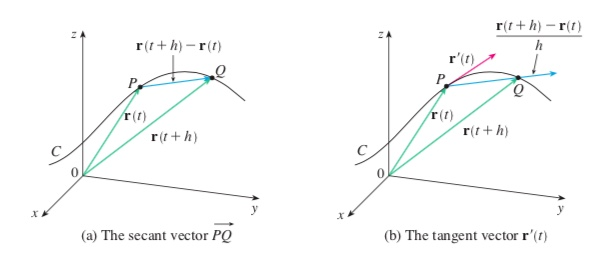
\includegraphics[scale=0.4]{figures_mvc/tangent_vector_secant_vector}
\end{center}
\caption{The derivative $\bbr'(t)$ is the tangent vector to the curve $\bbr$ at $\bbr(t)$.}
\end{figure}
The next theorem shows that we can compute the derivative of a vector-valued function in terms of the derivatives of its component functions.

\begin{thm}[Derivative of a vector-valued function]
	The derivative of a vector-valued function $\bbr(t)=(r_1(t),r_2(t),r_3(t))$ is given by 
	\begin{align*}
		\bbr'(t)=(r_1'(t),r_2'(t),r_3'(t)).
	\end{align*}
\end{thm}

\begin{pf}
By Theorem \ref{thm:limit_of_a_vector-valued_function}
\begin{align*}
	\bbr'(t)&=\lim_{h \to 0}\frac{\bbr(t+h)-\bbr(t)}{h} \\
	&=\lim_{h \to 0}\frac{(r_1(t+h),r_2(t+h),r_3(t+h))-(r_1(t),r_2(t),r_3(t))}{h} \\
	&=\lim_{h \to 0}\frac{(r_1(t+h)-r_1(t),r_2(t+h)-r_2(t),r_3(t+h)-r_3(t))}{h} \\
	&=\lim_{h \to 0}\left(\frac{r_1(t+h)-r_1(t)}{h},\frac{r_2(t+h)-r_2(t)}{h},\frac{r_3(t+h)-r_3(t)}{h}\right) \\
	&=\left(\lim_{h \to 0}\frac{r_1(t+h)-r_1(t)}{h},\lim_{h \to 0}\frac{r_2(t+h)-r_2(t)}{h},\lim_{h \to 0}\frac{r_3(t+h)-r_3(t)}{h}\right) \\
	&=(r_1'(t),r_2'(t),r_3'(t)).
\end{align*}	
\end{pf}

\fixme{Add examples.}

\begin{thm}[Differentiation formulas]
	Let $\bu,\bv$ be differentiable vector-valued functions into $\R^n$, $c$ a constant, and $\varphi:\mathbb{R} \to \mathbb{R}$ a real-valued function. Then
\begin{enumerate}[(1)]
		\item $[\bu(t)+\bv(t)]'=\bu'(t)+\bv'(t)$
		\item $[c\bu(t)]'=c\bu'(t)$
		\item $[\varphi(t)\bu(t)]'=\varphi'(t)\bu(t)+\varphi(t)\bu'(t)$
		\item $[\bu(t)\cdot \bv(t)]'=\bu'(t)\cdot \bv(t)+\bu(t) \cdot \bv'(t)$
		\item $[\bu(t)\times \bv(t)]'=\bu'(t)\times \bv(t)+\bu(t) \times \bv'(t)$ (for $n=3$)
		\item $[\bu(\varphi(t))]'=\varphi'(t)\bu'(\varphi(t))$
	\end{enumerate}	
\end{thm}

\begin{pf}
\fixme{Add proof.}	
\end{pf}


\begin{defn}[Higher derivatives]
	\begin{enumerate}[(a)]
		\item The \emph{second derivative}, $\bbr''$, of a vector-valued function $\bbr$ is the derivative of $\bbr'$: $\bbr''=(\bbr')'$. Thus,
\begin{align*}
	\bbr''(t)=(f''(t), g''(t), h''(t))
\end{align*}
Similarly, for $k$ a positive integer, the $k$th derivative of $\bbr$ is given by the formula
\begin{align*}
	\bbr^{(k)}(t)=(f^{(k)}(t), g^{(k)}(t), h^{(k)}(t)).
\end{align*}
\item A vector-valued function is said to be of class $\mathscr{C}^k$ if its first $k$ derivatives exist and are continuous and of class $\mathscr{C}^\infty$ if all of its derivatives exist. Functions in the class $\mathscr{C}^\infty$ are also called \emph{smooth}.
	\end{enumerate}
\end{defn}

\subsection{Parametrized Curves}
We will now focus on a special class of vector-valued functions, which model the motion of a particle through space. Throughout this section, let $I=(a,b)$ be an open interval in $\R$.

\begin{defn}[Parametrized curve]
	A \emph{parametrized curve} (or just \emph{curve}) is a smooth mapping $\bbr:I \to \mathbb{R}^n$. For $n=2$, a curve is also called a \emph{plane curve} while for $n=3$ it is also called a \emph{space curve}. The variable $t$ is called the \emph{parameter}. The image $\bbr(I)$ is called the \emph{trace} of the curve $\bbr$.
\end{defn}

\begin{example}
The graph of any function $y=f(x)$ can be written as a parametrized curve by defining
\begin{align*}
	\bbr:\R &\to \R^2 \\
	\bbr(t)&=(t,f(t)).
\end{align*}
For example, the function $y=x^2$ can be written the parametrized curve $\bbr(t)=(t,t^2)$ for all $-\infty < t < \infty$.	The trace of a plane curve can be plotted in \emph{Mathematica} as shown below:

\begin{figure}[h]
	\begin{center}
		\includegraphics[scale=0.5]{figures_mvc/parab_param_plot}
	\end{center}
	\caption{The trace of the plane curve $\bbr(t)=(t,t^2)$.}
\end{figure} 

The particle moves down the parabola from the upper left starting at $t=-\infty$, reaches the origin at $t=0$, and then continues up the parabola to the upper right for all $t>0$.
\end{example}

\begin{exercise}
Sketch the trace of the plane curve $\bbr(t)=(t^2-2t,t+1)$, $-\infty < t < \infty$ in by making a table of the coordinates $(x(t),y(t))$ for integer values of $t$ from $-2 \leq t \leq 4$. Compare your sketch with the curve produced in \emph{Mathematica} using the ``ParametricPlot" command.	
\end{exercise}
\newpage 
{\color{red}
\begin{solution}
	The curve is a parabola, which we can confirm by eliminating $t$ as follows. First, solve for $t$ in terms of $y$ to obtain
\begin{align*}
	y=t+1 \implies y-1=t.
\end{align*}
Substituting into $x(t)$ then gives $x$ in terms of $y$:
\begin{align*}
	x=t^2-2t=(y-1)^2-2(y-1)=y^2-4y+3=(y-2)^2-1.
\end{align*}
which is the equation of a parabola in vertex form, with vertex at $(x,y)=(-1,2)$. 

\begin{figure}[h]
	\begin{center}
		\includegraphics[scale=0.5]{figures_mvc/sideways_parab_mma}
	\end{center}
	\caption{The trace of the plane curve $\bbr(t)=(t^2-2t,t+1)$ from $-2 \leq t \leq 4$.}
\end{figure}

The particle travels upwards along the parabola from $t=-\infty$, reaches the vertex at $t=1$, and then continues upward to the right for $t>0$.
\end{solution}}

\begin{example}
Consider the following three plane curves
\begin{enumerate}[(1)]
	\item $\bbr_1(t)=(\cos t, \sin t), 0 \leq t \leq 2\pi$, 
	\item $\bbr_2(t)=(-\sin 2t, \cos 2t), 0 \leq t \leq 2\pi$,
	\item $\bbr_3(t)=(\cos(-t), \sin(-t)), 0 \leq t \leq 2\pi$.
\end{enumerate}	
For all three curves, $x(t)^2+y(t)^2=1$, so the trace of each curve is the unit circle. However, the curves are different. The reader can easily verify the following by making a table for each curve and sketching the trace:
\begin{enumerate}[(1)]
	\item In $\bbr_1$, the particle begins at $(x,y)=(1,0)$ at $t=0$ and completes one full circle, moving in the counterclockwise direction.
	\item In $\bbr_2$, the particle begins at $(x,y)=(0,1)$ at $t=0$ and completes \emph{two} full circles, moving in the counterclockwise direction.
	\item In $\bbr_3$, the particle begins at $(x,y)=(1,0)$ at $t=0$ and completes one full circle, moving in the \emph{clockwise} direction.
\end{enumerate}
\begin{figure}[h]
	\begin{center}
		\includegraphics[scale=0.4]{figures_mvc/circ_param_plot_mma}
	\end{center}
	\caption{The trace of the curves $\bbr_1,\bbr_2,\bbr_3$.}
\end{figure}
\end{example}
The previous example shows that a parametrized curve is more than just the trace: it is the trace together with a choice of how to traverse the trace of curve.

\begin{example}
Consider now the trace of the plane curve $\bbr(t)=(t^3,t^2)$, $-\infty<t<\infty$.

\begin{figure}[h]
	\begin{center}
		\includegraphics[scale=0.4]{figures_mvc/cusp_mma}
	\end{center}
\end{figure}
Since the component functions are smooth, the reader may be surprised by the cusp at the origin. Solving for $y$ in terms of $x$ by eliminating $t$, we find that $y=x^{2/3}$, which is indeed not differentiable at the origin. Note that $\bbr'(t)=(3t^2,2t)\neq (0,0)$ everywhere except the origin, where the tangent vector vanishes.
\end{example}
\newpage 
\begin{defn}[Regular curve]
	Let $\bbr:I \to \R^n$ be a parametrized curve.
	\begin{enumerate}[(a)]
		\item A point where $\bbr'(t)={\bf 0}$ is called a \emph{singular point}, while a point where $\bbr'(t) \neq {\bf 0}$ is called a \emph{regular point}.
		\item A \emph{regular curve} is a curve with no singular points; that is, it is a curve for whice $\bbr'(t) \neq {\bf 0}$ for all $t \in I$.
	\end{enumerate}
\end{defn}
In our study of the geometry of curves, we will need the curve to have a tangent vector at every point. Thus, from now on we will assume all curves are regular.



\end{document}

